\documentclass[xcolor=pdftex,dvipsnames,table,aspectratio=169]{beamer}
%\documentclass[xcolor=pdftex,dvipsnames,table,handout,aspectratio=169]{beamer}

%\setbeameroption{show notes}

\usepackage{bm,graphicx,multirow,amsmath,tikz} %fancybox,
\usepackage{color}%,textpos}
\usepackage[round]{natbib}
\usepackage[normalem]{ulem}
\usepackage{hyperref}
\usepackage{lastpage}
\usepackage{array}
\usepackage{color}
\usepackage{framed}
\usepackage{hyperref}

% Define Western colours
\definecolor{western}{rgb}{.306,.152,.524}
\definecolor{westerngray}{rgb}{.512,.508,.524}

%% Define BEAMER colours
\setbeamercolor{frametitle}{bg=western,fg=white}
\setbeamercolor{framesubtitle}{bg=western,fg=black}
\setbeamercolor{title}{fg=white,bg=western}
\setbeamercolor{author}{fg=white,bg=western}
\setbeamercolor{institute}{fg=white,bg=western}
\setbeamercolor{date}{fg=white,bg=western}

%% Set BEAMER fonts
\setbeamerfont{title}{shape=\bf}
\setbeamerfont{frametitle}{shape=\sc,size=\Large}
\setbeamerfont{framesubtitle}{shape=\sc,size=\Large}
\setbeamerfont{footline}{shape=\sc}

%% Define BEAMER toc
\setbeamercolor{section in toc}{fg=western}
\setbeamercolor{subsection in toc}{fg=westerngray}
\setbeamertemplate{sections/subsections in toc}[ball]

%% Define BEAMER background
\setbeamercolor{background canvas}{bg=white}

%% Define BEAMER footer
\setbeamertemplate{navigation symbols}{}
\setbeamercolor{footline}{fg=white,bg=western}
\setbeamertemplate{footline}{%
  \begin{beamercolorbox}[wd=\paperwidth]{footline}
    \vskip5pt

    \raisebox{.05in}{
      \scriptsize{\bf \insertshorttitle}
    }
    \hfill
    \raisebox{.05in}{
      \scriptsize{\bf \insertframenumber/\inserttotalframenumber} 
    }
    \hspace{5pt}

    \vskip5pt
  \end{beamercolorbox}
}

%% Define BLOCK environment
\setbeamercolor{block title}{fg=western}
\setbeamerfont{block title}{series=\bfseries}

%% Define ENUMERATE and ITEMIZE environements
\setbeamertemplate{itemize item}[ball]
\setbeamertemplate{enumerate item}[ball]
\setbeamercolor{item projected}{bg=western}

%% Define BEAMER toc
\setbeamercolor{sections/subsections in toc}{fg=blue!75}
\setbeamertemplate{sections/subsections in toc}[ball]

% %% Define SECTION openings
% \AtBeginSection[]{
%   \begin{frame}{\insertshorttitle}
%     \tableofcontents[currentsection,subsectionstyle=hide/hide/hide]
    
%   \end{frame}
% }

%% Define BEAMER frametitle
\addtobeamertemplate{frametitle}{
   \let\insertframetitle\insertsectionhead}{}
\addtobeamertemplate{frametitle}{
   \let\insertframesubtitle\insertsubsectionhead}{}


\makeatletter
  \CheckCommand*\beamer@checkframetitle{\@ifnextchar\bgroup\beamer@inlineframetitle{}}
  \renewcommand*\beamer@checkframetitle{\global\let\beamer@frametitle\relax\@ifnextchar\bgroup\beamer@inlineframetitle{}}
\makeatother

% Define counters for example and exercise
\newcounter{example}
\newcounter{exercise}

% Define example and exercise commands
\renewcommand{\example}
{\stepcounter{example}Example \lecturenum.\arabic{example}}
\newcommand{\examplectd}
{Example \lecturenum.\arabic{example}\ ctd}
\newcommand{\exercise}
{\stepcounter{exercise}Exercise \lecturenum.\arabic{exercise}}
\newcommand{\exercisectd}
{Exercise \lecturenum.\arabic{exercise}\ ctd}


\newcommand{\lecturenum}{9}

\title[SS2857]{Probability and Statistics I}
\subtitle{\lecturenum. Expected Values of Discrete Random Variables}

\date{}

% %% Add logo
% \titlegraphic{\includegraphics[height=2cm]{../uwo_logo_reversed}}

%% Initialize R


\begin{document}

{
\setbeamertemplate{footline}{}
\setbeamercolor{background canvas}{bg=western}

\begin{frame}
  \addtocounter{framenumber}{-1}

  \maketitle
\end{frame}
}

\begin{frame}
  \frametitle{\invisible{Hello}}

  \begin{center}
    \Large{\textbf{3.3 Expected Values of Discrete Random Variables}}
  \end{center}

  \begin{center}


  \end{center}
\end{frame}



\section{Expected Values of Discrete RVs}

\begin{frame}
  \begin{block}{Expected Value or Mean}
    Let $X$ be a discrete rv with set of possible values $D$ and pmf $p(x)$. 
    
    \medskip
    
    The expected value or mean value of $X$ is
    \[
      E(X)=\mu_X=\sum_{x\in D} xp(x).
    \]
    
    \medskip
    
    The expected value will exist provided that $\sum_{x\in D} |x|p(x) < \infty$. 

  \end{block}


\end{frame}

\section{Expected Values of Discrete RVs}

\begin{frame}
  \begin{block}{Expected Value or Mean: Interpretation}
    
  
    The expected value is the weighted average of all possible outcomes. It tells us about the centre of the distribution.
    
    \medskip
    It represents the limiting average of the random variable on repeated experiments. 
    
    \medskip
    
    If we were to repeat the same experiment many, many times and record the value of $X$ each time then the average of these values would be very close to $E(X)$ and get closer and closer the more times we repeat the experiment. 
  \end{block}
\end{frame}

\begin{frame}
  \begin{block}{Variance and Standard Deviation}
  
  Let $x$ be a possible value of $X$. The deviation associated with $x$ is
  $$
  x-\mu_X = x - E(X).
  $$
  
  \medskip
  \begin{itemize}
  \item A positive deviation indicates that $x > E(X)$.
  \item A negative deviation indicates that $x < E(X)$.
  \item The deviation increases in magnitude the farther $x$ is from $E(X)$. 
  \end{itemize}
  \end{block}
\end{frame}

\begin{frame}
  \begin{block}{Variance and Standard Deviation}
    Let $X$ be a discrete rv with set of possible values $D$ and pmf $X$. The variance of $X$ is
    \[
      V(X)=\sigma^2_X=\sum_{x\in D} (x-\mu_x)^2p(x)=E(X-\mu_X)^2.
    \]

    \vspace{-.2in}

    The standard deviation is $\sigma_X=\sqrt{\sigma^2_X}$.

  \end{block}
\end{frame}

\begin{frame}
  \begin{block}{Variance and Standard Deviation: Interpretation}
    The variance is the weighted average of all possible \textit{squared deviations}. It tells us about the spread of the distribution.
    
    \medskip
    It represents the limiting average of the \textit{squared deviation} on repeated experiments. 

  \end{block}
\end{frame}



\begin{frame}
  \begin{block}{\example}
  Compare the mean and variance of the distributions with the following pmfs.
  
  \begin{center}
    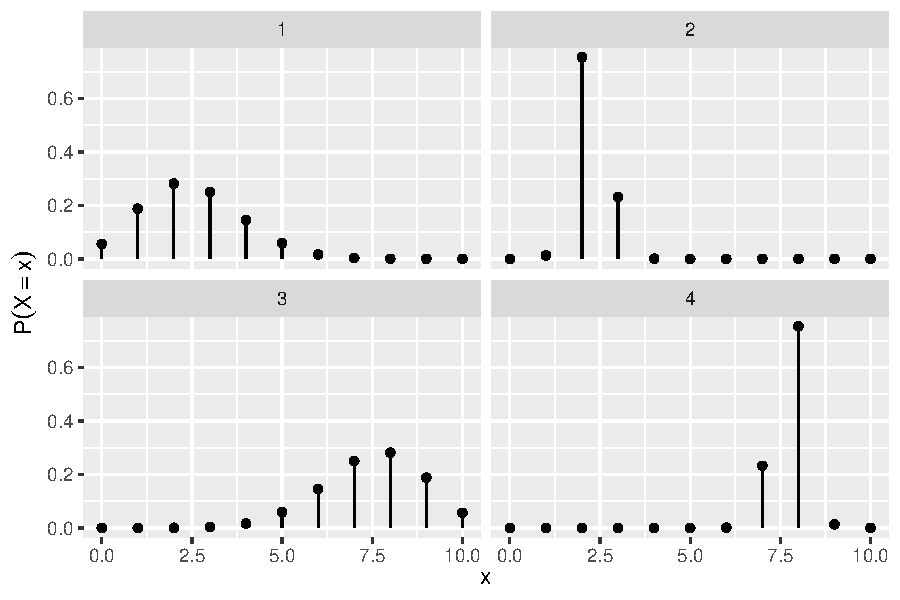
\includegraphics[height = .6\textheight]{figure/example-12-1-1-1}
  \end{center}
  \end{block}

\end{frame}

\begin{frame}

  \begin{block}{\example: Expected Values and Variances}

    Approximately 79\% of the world's population has brown eyes\footnote{\url{https://www.worldatlas.com}}.

    \medskip
    
    Suppose that we sample 5 people from the population at random with replacement and record their eye-colour as brown or not brown. Let $X$ represent the number of people in our sample with brown eyes.

    \medskip
    
    
    \begin{enumerate}[a)]
    \item Compute the expected value of $X$. 
    \item Compute the variance of $X$.
    \item Compute the standard deviation of $X$.
    \item Provide an interpretation for $E(X)$.
    \end{enumerate}
    
  \end{block}
  
\end{frame}

\begin{frame}
\begin{block}{\examplectd: Expected Values and Variances}
% latex table generated in R 4.4.1 by xtable 1.8-4 package
% Fri Oct  4 11:35:31 2024
\begin{table}[ht]
\centering
\begin{tabular}{rr}
  \hline
x & $p(x)$ \\ 
  \hline
     0 & 0.00041 \\ 
       1 & 0.00768 \\ 
       2 & 0.05780 \\ 
       3 & 0.21743 \\ 
       4 & 0.40898 \\ 
       5 & 0.30771 \\ 
   \hline
\end{tabular}
\end{table}

\end{block}
\end{frame}

\begin{frame}
\begin{block}{\examplectd: Expected Values and Variances}
% latex table generated in R 4.4.1 by xtable 1.8-4 package
% Fri Oct  4 11:35:31 2024
\begin{table}[ht]
\centering
\begin{tabular}{rrr}
  \hline
x & $p(x)$ & $x - \mu_X$ \\ 
  \hline
     0 & 0.00041 & -3.95000 \\ 
       1 & 0.00768 & -2.95000 \\ 
       2 & 0.05780 & -1.95000 \\ 
       3 & 0.21743 & -0.95000 \\ 
       4 & 0.40898 & 0.05000 \\ 
       5 & 0.30771 & 1.05000 \\ 
   \hline
\end{tabular}
\end{table}

\end{block}
\end{frame}

\begin{frame}
  \begin{block}{General Functions of Random Variables}

    Generally, the random variable $Y$ is a function of $X$ if
    \[
      Y=h(X)
    \]
    for some function $h(\cdot)$. 

    \medskip

    If this is true then
    \begin{align*}
      E(Y)&=E[h(X)]=\sum_{x \in D}h(x)p(x)\\
      V(Y)&=V[h(X)]=\sum_{x \in D}\left(h(x) - E[h(X)]\right)^2 p(x)
    \end{align*}
  \end{block}
\end{frame}

\begin{frame}
  \begin{block}{Linear Functions of Random Variables}

    We say that the random variable $Y$ is a linear function of $X$ if
    \[
      Y=a X + b
    \]
    for some constants $a,b \in \mathbb R$.

    \medskip

    If this is true then
    \begin{align*}
      E(Y)&=E(aX + b)=aE(X) + b\\
      V(Y)&=V(aX + b)=a^2V(X)\\
      SD(Y)&=SD(aX + b)=|a|SD(X).
    \end{align*}
  \end{block}
\end{frame}

\begin{frame}

  \begin{block}{\example}
    Approximately 79\% of the world's population has brown eyes\footnote{\url{https://www.worldatlas.com}}.

    \medskip
    
    Suppose that we sample 5 people from the population at random with replacement and record their eye-colour as brown or not brown. Let $Y$ represent the number of brown eyes in the sample plus the number of hands\footnote{We'll assume that everyone has two of each}.

    \medskip

    \begin{enumerate}[a)]
    \item Compute the expected value of $Y$. 
    \item Compute the variance of $Y$.
    \item Compute the standard deviation of $Y$.
    \item Provide an interpretation for $E(Y)$.
    \end{enumerate} 
  \end{block}
\end{frame}

\begin{frame}

  \begin{center}
    \Large{\textbf{Questions?}}
  \end{center}
\end{frame}

\begin{frame}
  \begin{block}{\exercise}
  
  A professor driving to Western must pass through 5 sets of traffic lights. There is a .75 percent chance of being stopped at each light (or so it appears to him). The time it takes him to complete the drive is 15 minutes plus 3 minutes for each light he has to stop at. 

    Let $X$ be the number of lights he must stop at and $Y$ the time it takes him in minutes.
    \begin{enumerate}[a)]
    \item Compute the expected value, variance, and standard deviation of $X$.
    \item Provide an interpretation for the expected value.
    \item Compute the expected value, variance, and standard deviation of $Y$.
    \end{enumerate}
  \end{block}
\end{frame}

\end{document}
